%%%%%%%%%%%%%%%%%%%%%%%%%%%%%%%%%%%%%%%%%%%%%%%%%%%%%%%%%%%%%%%%%%%%%%%%%%%%%%%%
%%%%%%%%%%%%%%%%%%%%%%%%%%%%%%%%%%%%%%%%%%%%%%%%%%%%%%%%%%%%%%%%%%%%%%%%%%%%%%%%
%%%%%%%%%%%%%%%%%%%%%%%%%%%%%%%%%%%%%%%%%%%%%%%%%%%%%%%%%%%%%%%%%%%%%%%%%%%%%%%%
\chapter[Medida de la fase $\phis$ en el canal $\Bs \rightarrow \text{J}/\uppsi \antikaon\kaon$][Medida de la fase ${\textit{φ}}_{\text{s}}$ en el canal $\bm{\Bs \rightarrow \text{J/}}\text{ψ}  \bm{\antikaon\kaon}$]{Medida de la fase ${\textit{φ}}_{\text{s}}$ en el canal $\bm{\Bs \rightarrow \text{J/}}\text{ψ}  \bm{\antikaon\kaon}$}
\label{cha:ana}
%%%%%%%%%%%%%%%%%%%%%%%%%%%%%%%%%%%%%%%%%%%%%%%%%%%%%%%%%%%%%%%%%%%%%%%%%%%%%%%%
%%%%%%%%%%%%%%%%%%%%%%%%%%%%%%%%%%%%%%%%%%%%%%%%%%%%%%%%%%%%%%%%%%%%%%%%%%%%%%%%
%%%%%%%%%%%%%%%%%%%%%%%%%%%%%%%%%%%%%%%%%%%%%%%%%%%%%%%%%%%%%%%%%%%%%%%%%%%%%%%%


En términos generales, cabe señalar unas ideas generales a tener en cuenta a la hora de medir la fase electrodébil $\phis$:
\begin{itemize}
    \item El rango de tempo de decaimiento es $t\in[0.3,15]$ ps. La cota inferior suprime mucho fondo combinatorio, mientras que la cota superior es debida a que ya no hay casi eventos a partir de $15$ ps.
  \item Se ajusta el valor $\Gamma_s - \Gamma_d$, debido a que puede ser medido independientemente del valor de $\Gamma_d$, resolviéndose mejor que si se ajustase $\Gamma_s$ directamente.
  \item Se asume que no hay dependencia entre los ratios \textit{penguin}--árbol, tomando por tanto un único $\lambda$ para todas las polarizaciones.
  \item El rango de masa del ajuste está limitado a la región de masa $m_{\text{KK}} = [990,1050]$ MeV alrededor de la resonancia del $\fai$ y dominada por ella, que se subdividide en seis bines de masa.
  \item No se tendrá en cuenta el $D$ wave en este análisis, porque es despreciable en este análisis, al ser su contribución a ala ventana de masa muy pequeña. El conjunte de factores $C_{SP}$ empleado es $$ C_{\text{SP}}  = \{0.8463,0.8756,0.8478,0.8833,0.9415,0.9756\}.$$
  \item Al tratar con \emph{full} MC o datos, cada evento $i$ está pesado con una ponderación de señal, $w_i$, obtenida mediante el método ${}_s$\textit{Plot}. De este modo se elimina el ruido y solo se modela la señal. La verosimilitud en cada muestra se escala por un factor $w_i \,\frac{\sum w_i}{\sum w_i^2}$, para tener en cuenta los pesos en las incertidumbres de los parámetros.
\end{itemize}





%\section{Decay time acceptance}
%
%The decay time acceptance is defined as
%\begin{equation}
%  \epsilon_{\text{data}}^{\Bs} = \epsilon_{\text{data}}^{\text{B}{}_{\text{d}}^0} \times  \frac{\epsilon_{\text{MC}}^{\text{B}{}_{\text{s}}^0}}{\epsilon_{\text{MC}}^{\text{B}{}_{\text{d}}^0}}
%\end{equation}
%
%
%...
%
%This acceptance is modelled with cubic b--splines with the first coefficient fixed to unity. In order to fix the basis $k$ is defined
%\[k = \{0.3, 0.58, 0.91, 1.35, 1.96, 3.01,7.00\}\]
%which is a set of knots exponentialy distributed, thus having six equally distributed time bins.
%There exist three splines following splines  (one per dataset).
%
%In order to model the resolution, a Gaussian of zero-mean and standard deviation $\sigma$ is used. After the studies of time resolution, the values obtained for each dataset for $\sigma$ are the ones of Table \ref{tab_dectimeacc}.
%
%\begin{table}[H]
%\centering
%\begin{tabular}{lccc} \toprule
%& $\Bs$ MC sample & $\text{B}{}_{\text{d}}^0$ MC sample & $\text{B}{}_{\text{d}}^0$ data sample \\ \midrule
%$\sigma$ (ps) & $41.7$ & $38.64$ & $42.44$ \\
%$\Gamma \, \mathrm{(ps^{-1})}$ & $0.6613701$ & $0.65833$ & $0.65789$ \\
%\bottomrule
%\end{tabular}  
%\caption{Values of resolution and lifetime for each sample.} \label{tab_dectimeacc}
%\end{table} 
%
%
%
%
%
%For each sample, data an MC, the model used for the ajuste is composed of a single-tail exponential convoluted with a single Gaussian resolution, multiplied by the acceptance function, i.e., the b-splines.
%
%
%
%Let $b$ be the set of coefficients of the spline. Since cubic b-splines are used with a set of 6+1 knots, $b$ is a nine-dimensional set of parameters,
%\begin{equation}
%  b = \{1,b_1,b_2,b_3,b_4,b_5,b_6,b_7,b_8\}
%\end{equation} 
%Let also $s$ be the cubic b-spline defined for a given tine bin,
%\begin{equation}
%  s = c_0 + c_1 t + c_2 t^2 + c_3 t^3
%\end{equation}
%that depends on four coefficients, that are indeed functions of $b$ coefficients, $c_i = c_i(b)$.
%At de last knot, a linear extrapolation is done up to $t = 15$ ps. To achieve this, the two following conditions are imposed:
%\[f(7) = g(7) \qquad f'(7) = g'(7) \]
%being $f$ the function before $t=7$ and $g$ the one for higher values.
%
%
%
%
%By the other hand, the right-tail exponential distibution and the resolution gaussian are
%\[E(t;\Gamma) = \Gamma e^{-\Gamma t}
%\qquad 
%G(t;\sigma) = \frac{e^{-\frac{t^2}{2 \sigma^2}}}{\sqrt{2 \pi } \sigma}.\]
%
%The convolution between exponential and gaussian is analytical, it is found to be:
%\begin{equation}
%\begin{split}
%    G * E &= \int_0^{\infty} E(t-x;\Gamma) G(x;\sigma) dx\\ &= \frac{1}{2} e^{\frac{1}{2} \Gamma \left(\Gamma \sigma^2-2 t\right)} \text{erfc}\left(\frac{\Gamma \sigma-\frac{t}{\sigma}}{\sqrt{2}}\right)
%\end{split}
%\end{equation}
%
%So, it only remains to multiply by the spline, $s$, being the p.d.f. function to ajuste \textbf{on each bin},
%\begin{equation}
% f(t;\Gamma,\sigma,c_i)) =  (E * G) \times (c_0 + c_1 t + c_2 t^2 + c_3 t^3)
%\end{equation}
%which integral is also analylic and can be computed with a CAS.
%When fitting $c_i$ parameters must be obtained on the fly by a transation between $b$, taking into account the value of $t$ at the event, since they are bin--dependent.
%
%
%In order to obtain the $s_{\text{data}}^{\Bs} $ spline, a simultaneous 3--step ajuste is performed:
%\begin{itemize}
%  \item First $\Bs$ MC sample is fitted obtaining $s_{\text{MC}}^{\Bs} $.
%  \item Second, $(E*G) \times s_{\text{MC}}^{\Bs} \times s_{\text{MC}}^{\mathrm{B_d^0}/\Bs} $ is fitted against $\mathrm{B_d^0}$ MC sample taking $s_{\text{MC}}^{\Bs} $ from previous step.
%  \item Finally, $(E*G) \times s_{\text{MC}}^{\mathrm{B_d^0}/\Bs} \times s_{\text{data}}^{\Bs} $ is fitted against $\mathrm{B_d^0}$ data sample taking $s_{\text{MC}}^{\mathrm{B_d^0}/\Bs} $ from previous step.
%\end{itemize}
%


%%%%%%%
%%%%%%%
%%%%%%%
%%%%%%%
%%%%%%%
%%%%%%%
%%%%%%%
%%%%%%%










\section{Determinación de la aceptancia en el tiempo de desintegración}

La eficiencia de reconstrucción no es constante como función de la vida media del $\Bs$ debido a dos factores: los requerimientos de desplazamiento hechos en las trazas de señal en el \emph{trigger} y la selección de eventos; y a la propia eficiencia de reconstrucción de las trazas en el VELO CITAR 24. La aceptancia en el tiempo de desintegración es determinada usando el canal de control $B_d \rightarrow \Jpsi \text{K}{}^{*0}(892)(\rightarrow \antikaon \uppi^-)$, que es cinemáticamente muy similar a la señal y se asume que tiene una distribución de decaimiento puramente exponencial, se desprecia la anchura $\Delta \Gamma _d$ con una vida media muy bien conocida. \cite{paperPhis}

Se define la aceptancia en el tiempo de desintegración, $ \epsilon_{\text{data}}^{\Bs} $, como
\begin{equation}
  \epsilon_{\text{data}}^{\Bs} = \epsilon_{\text{data}}^{\text{B}{}_{\text{d}}^0} \times  \frac{\epsilon_{\text{MC}}^{\text{B}{}_{\text{s}}^0}}{\epsilon_{\text{MC}}^{\text{B}{}_{\text{d}}^0}}
\end{equation}
donde $\epsilon_{\text{data}}^{\text{B}{}_{\text{d}}^0}$ es la eficiencia para los eventos totalmente \textit{triggered}, seleccionados y s--ponderados en el canal de control $\text{B}{}_{\text{d}}^0$; y $r(t) = \sfrac{\epsilon_{\text{MC}}^{\text{B}{}_{\text{s}}^0}}{\epsilon_{\text{MC}}^{\text{B}{}_{\text{d}}^0}}$ el cociente de las eficiencias entre los MC. De este modo, el cociente entre MC toma en cuenta las pequeñas diferencias entre la vida media y cinemática entre los modos de señal y control entre los dos MC, mientras que los datos de $B_d$ corrigen las diferencias entre los MC y los datos de $\Bs$.

La línea de trabajo consiste en hacer un ajuste simultáneo a las tres muestras de datos de forma que se pueda derivar $\epsilon_{\text{data}}^{\Bs} $, siendo de este modo posible conseguir una correcta estimación de las incertidumbres en los coeficientes de la aceptancia. Esta aceptancia es después usada para obtener los parámetros físicos de la desintegración del $\Bs$.

Esta aceptancia está modelada con b--splines cúbicos con el primer coeficiente fijado a la unidad. Para fijar la base se define $k$,
\[k = \{0.3, 0.58, 0.91, 1.35, 1.96, 3.01,7.00\}\]
un conjunto de nudos exponencialmente distribuidos, teniendo por lo tanto seis bines \emph{quasi}--equipoblados. Existen de este modo $3$ splines, uno para cada conjunto de datos, que son:
\begin{itemize}
	\item $s_{\text{MC}}^{\Bs}$, que representa la aceptancia de la desintegración del MC de $\Bs$.
	\item $s_{\text{MC}}^{\mathrm{B_0}/\Bs}$, que representa el cociente entre las aceptancias de los MC.
	\item $s_{\text{data}}^{\Bs}$, el b--spline buscado, que representa la aceptancia de los datos $\Bs$. 
\end{itemize}


A la hora modelar la resolución del detector del tiempo de desintegración, se emplea una gaussiana de media cero y desviación típica $\sigma$. Después de los estudios de resolución temporal, los valores obtenidos para $\sigma$ de cada conjunto de datos son los mostrados el la Tabla \ref{tab_dectimeacc}.
Para cada muestra, tanto de datos como de MC, el modelo usado para el ajuste está compuesto de una distribución exponencial de una cola convolucionada con una gaussiana simple de resolución, multiplicada por la función de aceptancia, i.e., los b--splines.

\begin{table}[H]
\centering
\begin{tabular}{lccc} \toprule
& muestra $\Bs$ MC  & muestra $\text{B}{}_{\text{d}}^0$ MC  & muestra $\text{B}{}_{\text{d}}^0$ datos \\ \midrule
$\sigma$ (ps) & $41.7$ & $38.64$ & $42.44$ \\
$\Gamma \, \mathrm{(ps^{-1})}$ & $0.6613701$ & $0.65833$ & $0.65789$ \\
\bottomrule
\end{tabular}  
\caption{Valores de la resolución y vida media para cada muestra \cite{amhis2017averages}.} \label{tab_dectimeacc}
\end{table} 







Dado que se emplean b-splines cúbicos con un conjunto de $6+1$ nudos, el conjunto de parámetros que definen el spline será un conjunto $b$ con $6+3=9$ parámetros que han de ser calculados para que el spline interpole a los datos,
\begin{equation}
  b = \{1,b_1,b_2,b_3,b_4,b_5,b_6,b_7,b_8\}.
\end{equation} 
Considerando $s$ el b--spline cúbico definido para un bin de tiempo dado,
\begin{equation}
  s = \beta_0 + \beta_1 t + \beta_2 t^2 + \beta_3 t^3
\end{equation}
que depende de cuatro coeficientes, que de hecho son funciones de los coeficientes $b$, $\beta_i = \beta_i(b)$.

En el último nudo se hace una extrapolación lineal hasta $t=15$ ps. Para lograr esto, se imponen dos condiciones, 
\[f(t=7 \text{ ps}) = g(t=7 \text{ ps}) \qquad f'(t=7 \text{ ps}) = g'(t=7 \text{ ps}) \]
siendo $f$ la función antes de $t=7$ ps y $g$ la que se encuentra a la derecha.


Por otra parte, la distribución exponencial y la distribución gaussiana toman la forma
\[E(t;\Gamma) = \Gamma e^{-\Gamma t}
\qquad 
G(t;\sigma) = \frac{e^{-\frac{t^2}{2 \sigma^2}}}{\sqrt{2 \pi } \sigma}.\]
La convolución entre exponencial y gaussiana es analítica, y se encuentra que
\begin{equation}
\begin{split}
    G * E &= \int_0^{\infty} E(t-x;\Gamma) G(x;\sigma) dx\\ &= \frac{1}{2} e^{\frac{1}{2} \Gamma \left(\Gamma \sigma^2-2 t\right)} \text{erfc}\left(\frac{\Gamma \sigma-\frac{t}{\sigma}}{\sqrt{2}}\right).
\end{split}
\end{equation}
%
De este modo solo resta multiplicar el spline, $s$, siendo la función \textit{p.d.f.} para ajustar en cada bin de tiempo,
\begin{equation}
 f(t;\Gamma,\sigma,\beta_i) =  (E * G) \times (\beta_0 + \beta_1 t + \beta_2 t^2 + \beta_3 t^3)
\end{equation}
cuya integral es también analítica y puede calcularse con un sistema CAS. A la hora de ajustar los parámetros $\beta_i$, estos deben ser obtenidos mediante una transformación entre ellos y el conjunto $b$, tomando en consideración el valor de $t$, puesto que son dependientes del bin.

En aras de obtener la aceptancia en el tiempo, $s_{\text{data}}^{\Bs} $, se realiza un ajuste simultáneo a las tres muestras y que consta de tres pasos:
\begin{itemize}
  \item Se ajusta $(E*G) \times s_{\text{MC}}^{\Bs}$  con la muestra de $\Bs$ MC, de modo que se obtienen los coeficientes, $b_i$, del spline $s_{\text{MC}}^{\Bs} $.
  \item Se ajusta $(E*G) \times s_{\text{MC}}^{\Bs} \times s_{\text{MC}}^{\mathrm{B_d^0}/\Bs} $ con los datos de la muestra $\mathrm{B_d^0}$ tomando por fijos los parámetros del spline $s_{\text{MC}}^{\Bs} $ del paso previo y obteniendo los coeficientes $r_i$.
  \item Finalmente, $(E*G) \times s_{\text{MC}}^{\mathrm{B_d^0}/\Bs} \times s_{\text{data}}^{\Bs} $ se ajusta con la muestra de datos $\mathrm{B_d^0}$, se toma el spline $s_{\text{MC}}^{\mathrm{B_d^0}/\Bs} $ del paso anterior y se obtiene el conjunto de coeficientes $c_i$.
\end{itemize}
%
Las tres fases se realizan simultáneamente, y se emplean tanto datos como MC de 2016 en la categorías de trigger \texttt{biased} y \texttt{unbiased} (\textit{vid.} \S \ref{sec_hltrigger}).


El actual algoritmo en uso para realizar este ajuste y obtener los coeficientes del spline de aceptancia está escrito en \texttt{C++} y corre sobre CPU, con un tiempo estimado de 30 minutos para ajustar las dos categorías de \textit{trigger} para 2015 y 2016. Para reducir el tiempo de ajuste y acelerar el análisis, se implementó este algoritmo en GPU, siendo capaz de correr en 6 minutos el mismo ajuste a las cuatro, ya mencionadas, muestras de datos.

El conjunto de coeficientes obtenidos que modelan la aceptancia en el tiempo de desintegración del $\Bs$,
 se muestran en la Tablas \ref{tab:acctimebsdataunbiased2016} y \ref{tab:acctimebsdatabiased2016}, y puede verse el gráfico de los ajustes en las Figuras \ref{fig:acctimebsdataunbiased2016} y \ref{fig:acctimebsdatabiased2016}. Además en las Figuras \ref{fig:acctimeotherbiased2016} y \ref{fig:acctimeotherunbiased2016} pueden verse los ajustes a cada una de las muestras por separado, y también el cociente entre MC's, junto con las proyecciones de los splines correspondientes.

\begin{table}[H]
\centering
\begin{multicols}{3}

\begin{tabular}{cc}
\toprule 
\multicolumn{2}{c}{$s_{\text{MC}}^{\Bs}$} \\ \midrule
$ b_0^{\text{BsMC}} $&$   1                  $\\
$ b_1^{\text{BsMC}} $&$   1.603 \pm 0.032    $\\
$ b_2^{\text{BsMC}} $&$   2.129 \pm 0.029    $\\
$ b_3^{\text{BsMC}} $&$   2.279 \pm 0.034    $\\
$ b_4^{\text{BsMC}} $&$   2.363 \pm 0.032    $\\
$ b_5^{\text{BsMC}} $&$   2.455 \pm 0.034    $\\
$ b_6^{\text{BsMC}} $&$   2.508 \pm 0.041    $\\
$ b_7^{\text{BsMC}} $&$   2.506 \pm 0.038    $\\
$ b_8^{\text{BsMC}} $&$   2.487 \pm 0.034    $\\
\bottomrule
\end{tabular}

\begin{tabular}{cc}
\toprule 
\multicolumn{2}{c}{$s_{\text{MC}}^{\mathrm{B_0}/\Bs}$} \\ \midrule
$ r_0^{\phantom{B}} $&$   1                  $\\
$ r_1^{\phantom{B}} $&$   0.924 \pm 0.027    $\\
$ r_2^{\phantom{B}} $&$   0.891 \pm 0.017    $\\
$ r_3^{\phantom{B}} $&$   0.871 \pm 0.019    $\\
$ r_4^{\phantom{B}} $&$   0.862 \pm 0.017    $\\
$ r_5^{\phantom{B}} $&$   0.846 \pm 0.017    $\\
$ r_6^{\phantom{B}} $&$   0.865 \pm 0.021    $\\
$ r_7^{\phantom{B}} $&$   0.823 \pm 0.019    $\\
$ r_8^{\phantom{B}} $&$   0.817 \pm 0.017    $\\
\bottomrule
\end{tabular}

\begin{tabular}{cc}
\toprule 
\multicolumn{2}{c}{$s_{\text{data}}^{\Bs}$} \\ \midrule
$ c_0^{\phantom{B}} $&$   1                  $\\
$ c_1^{\phantom{B}}  $&$   1.511 \pm 0.085    $\\
$ c_2^{\phantom{B}}  $&$   2.107 \pm 0.078    $\\
$ c_3^{\phantom{B}}  $&$   2.136 \pm 0.089    $\\
$ c_4^{\phantom{B}}  $&$   2.331 \pm 0.087    $\\
$ c_5^{\phantom{B}}  $&$   2.326 \pm 0.089    $\\
$ c_6^{\phantom{B}}  $&$   2.48  \pm 0.11     $\\
$ c_7^{\phantom{B}}  $&$   2.27  \pm 0.10     $\\
$ c_8^{\phantom{B}}  $&$   2.343 \pm 0.090    $\\
\bottomrule
\end{tabular}

\end{multicols}
\caption{Valores de los coeficientes de los b--splines que modelan la aceptancia en el tiempo de desintegración para la categoría de trigger \texttt{biased2016}.} \label{tab:acctimebsdatabiased2016}
\end{table}


\begin{table}[H]
\centering
\begin{multicols}{3}

\begin{tabular}{cc}
\toprule 
\multicolumn{2}{c}{$s_{\text{MC}}^{\Bs}$} \\ \midrule
$ b_0^{\text{BsMC}} $&$   1                  $\\
$ b_1^{\text{BsMC}} $&$   1.603 \pm 0.032    $\\
$ b_2^{\text{BsMC}} $&$   2.129 \pm 0.029    $\\
$ b_3^{\text{BsMC}} $&$   2.279 \pm 0.034    $\\
$ b_4^{\text{BsMC}} $&$   2.363 \pm 0.032    $\\
$ b_5^{\text{BsMC}} $&$   2.455 \pm 0.034    $\\
$ b_6^{\text{BsMC}} $&$   2.508 \pm 0.041    $\\
$ b_7^{\text{BsMC}} $&$   2.506 \pm 0.038    $\\
$ b_8^{\text{BsMC}} $&$   2.487 \pm 0.034    $\\
\bottomrule
\end{tabular}

\begin{tabular}{cc}
\toprule 
\multicolumn{2}{c}{$s_{\text{MC}}^{\mathrm{B_0}/\Bs}$} \\ \midrule
$ r_0^{\phantom{B}} $&$   1                  $\\
$ r_1^{\phantom{B}} $&$   0.924 \pm 0.027    $\\
$ r_2^{\phantom{B}} $&$   0.891 \pm 0.017    $\\
$ r_3^{\phantom{B}} $&$   0.871 \pm 0.019    $\\
$ r_4^{\phantom{B}} $&$   0.862 \pm 0.017    $\\
$ r_5^{\phantom{B}} $&$   0.846 \pm 0.017    $\\
$ r_6^{\phantom{B}} $&$   0.865 \pm 0.021    $\\
$ r_7^{\phantom{B}} $&$   0.823 \pm 0.019    $\\
$ r_8^{\phantom{B}} $&$   0.817 \pm 0.017    $\\
\bottomrule
\end{tabular}

\begin{tabular}{cc}
\toprule 
\multicolumn{2}{c}{$s_{\text{data}}^{\Bs}$} \\ \midrule
$ c_0^{\phantom{B}} $&$   1                  $\\
$ c_1^{\phantom{B}} $&$   1.511 \pm 0.085    $\\
$ c_2^{\phantom{B}} $&$   2.107 \pm 0.078    $\\
$ c_3^{\phantom{B}} $&$   2.136 \pm 0.089    $\\
$ c_4^{\phantom{B}} $&$   2.331 \pm 0.087    $\\
$ c_5^{\phantom{B}} $&$   2.326 \pm 0.089    $\\
$ c_6^{\phantom{B}} $&$   2.48  \pm 0.11     $\\
$ c_7^{\phantom{B}} $&$   2.27  \pm 0.10     $\\
$ c_8^{\phantom{B}} $&$   2.343 \pm 0.090    $\\
\bottomrule
\end{tabular}

\end{multicols}
\caption{Valores de los coeficientes de los b--splines que modelan la aceptancia en el tiempo de desintegración para la categoría de trigger \texttt{unbiased2016}.} \label{tab:acctimebsdataunbiased2016}
\end{table}

\todo[inline]{fix axes labels}

\newpage
\vspace*{\fill}
\begin{figure}[H]
\centering
\includegraphics[width=0.9\textwidth]{plots/decay_plots/unbiased2016/BdData_DecayTime_total}
\includegraphics[width=0.9\textwidth]{plots/decay_plots/unbiased2016/BdData_Spline_total}
\caption{Ajuste de la aceptancia en el tiempo de desintegración (arriba) y la función de aceptancia (abajo) para la categoría de trigger \texttt{unbiased2016}.}  \label{fig:acctimebsdataunbiased2016}
\end{figure}
\vspace*{\fill}
\newpage

\begin{figure}[H]
\centering
\begin{multicols}{2}
\includegraphics[width=\columnwidth]{plots/decay_plots/unbiased2016/BsMC_DecayTime_single}
\includegraphics[width=\columnwidth]{plots/decay_plots/unbiased2016/BdMC_DecayTime_single}
\includegraphics[width=\columnwidth]{plots/decay_plots/unbiased2016/BdData_DecayTime_single}
\includegraphics[width=\columnwidth]{plots/decay_plots/unbiased2016/BdMC_DecayTime_ratio}
\includegraphics[width=\columnwidth]{plots/decay_plots/unbiased2016/BsMC_Spline_single}
\includegraphics[width=\columnwidth]{plots/decay_plots/unbiased2016/BdMC_Spline_single}
\includegraphics[width=\columnwidth]{plots/decay_plots/unbiased2016/BdData_Spline_single}
\includegraphics[width=\columnwidth]{plots/decay_plots/unbiased2016/BdMC_Spline_ratio}
\end{multicols}
\caption{Ajustes de la aceptancia en el tiempo de desintegración (izquierda) y la función de aceptancia (derecha) para cada una de las tres muestras y para el cociente entre MC de la categoría de trigger \texttt{unbiased2016}.}  \label{fig:acctimeotherunbiased2016}
\end{figure}


\begin{figure}[H]
\centering
\includegraphics[width=0.9\textwidth]{plots/decay_plots/biased2016/BdData_DecayTime_total}
\includegraphics[width=0.9\textwidth]{plots/decay_plots/biased2016/BdData_Spline_total}
\caption{Ajuste de la aceptancia en el tiempo de desintegración (arriba) y la función de aceptancia (abajo) para la categoría de trigger \texttt{biased2016}.}  \label{fig:acctimebsdatabiased2016}
\end{figure}


\begin{figure}[H]
\centering
\begin{multicols}{2}
\includegraphics[width=\columnwidth]{plots/decay_plots/biased2016/BsMC_DecayTime_single}
\includegraphics[width=\columnwidth]{plots/decay_plots/biased2016/BdMC_DecayTime_single}
\includegraphics[width=\columnwidth]{plots/decay_plots/biased2016/BdData_DecayTime_single}
\includegraphics[width=\columnwidth]{plots/decay_plots/biased2016/BdMC_DecayTime_ratio}
\includegraphics[width=\columnwidth]{plots/decay_plots/biased2016/BsMC_Spline_single}
\includegraphics[width=\columnwidth]{plots/decay_plots/biased2016/BdMC_Spline_single}
\includegraphics[width=\columnwidth]{plots/decay_plots/biased2016/BdData_Spline_single}
\includegraphics[width=\columnwidth]{plots/decay_plots/biased2016/BdMC_Spline_ratio}
\end{multicols}
\caption{Ajustes de la aceptancia en el tiempo de desintegración (izquierda) y la función de aceptancia (derecha) para cada uno de las tres muestras y para el cociente entre MC de la categoría de trigger \texttt{biased2016}.}  \label{fig:acctimeotherbiased2016}
\end{figure}



\section{Ajuste a la distribución angular}


\subsection{Escáner de parámetros}

Es conocido que los algoritmos de minimización basados en gradiente, como es el caso de \textsc{Minuit}, pueden devolver un mínimo local. Para estudiar el perfil de la verosimilitud se practican escáneres de parámetros en un rango amplio alrededor del valor nominal del ajuste, podrían observarse mínimos adyacentes, y de ese modo corroborar que el nominal es el menor de los más próximos.

Se llevan a cabo escáneres de todos los parámetros involucrados en el ajuste, como pueden verse en las Figuras \ref{fig:scansmc}. Todos ellos resultaron apoyar que el mínimo nominal devuelto por \textsc{Minuit} era el menor, viendo por tanto que estamos en el máximo de la verosimilitud.









\section{Estudio de sistemáticos}

\subsection{Bias del ajuste}
\label{sec:fitbias}

El algoritmo empleado para ajustar los datos al modelo de distribución angular que desacopla las amplitudes de polarización y permite obtener los valores de $\phis$, así como $\Delta \Gamma$ y $\Gamma_{\text{s}} - \Gamma_{\text{d}}$, presenta, como sucede en todos los casos, un bias intrínseco y que da lugar a una incertidumbre sistemática en los parámetros.

Para estimar este bias se hacen $10^4$ realizaciones de $107628$ eventos cada una, por ser esta la señal efectiva real en 2015 y 2016. Para ello se toman como parámetros para la simulación los resultados del ajuste nominal \cite{paperPhis}, empleando como generador el mismo modelo respecto del cual serán ajustados. En esta primera versión del generador no se incluyen fenómenos de aceptancia temporal ni angular, solo estaría incluida la distribución angular y del tiempo.
%TODO mirar pulls

Los \textit{pulls} 
\begin{equation}
  \text{pull(par)} = \mathrm{ \frac{ par_{fit}^{value} - par_{gen}^{value} }{ par_{fit}^{uncertainty} } }
\end{equation}
y residuos,
\begin{equation}
  \text{residual(par)} = \mathrm{  par_{fit}^{value} - par_{gen}^{value} } 
\end{equation}
para cada uno de los parámetros que varían en el ajuste se muestran en la Figura \ref{tab:residfitbias}. Dado que se supone que la distribución de pulls será una normal de media cero y desviación típica unidad, y la de residuos será una gaussiana, se practican ajustes a sendas distribuciones. Finalmente en la Tabla \ref{tab:residfitbias}, la media del pull y su incertidumbre son sumadas en cuadratura y asignadas como un sistemático a cada parámetro. 

\begin{table}[H]
  \centering
  \begin{tabular}{cccc}
  \toprule
  Parámetro & $\mu$ & $\sigma$ & $u_{\mathrm{syst}}$\\ 
  \midrule
$\Delta \Gamma$ &  $-0.000078 \pm 0.000075$ &  $0.007451 \pm 0.000053$ & $ 0.00011 $\\
$\Gamma_{\mathrm{s}} - \Gamma_{\mathrm{d}}$ &  $0.000064 \pm 0.000024$ &  $0.002357 \pm 0.000017$ & $ 0.000068 $\\
$\Delta M$ &  $0.000021 \pm 0.000064$ &  $0.006386 \pm 0.000045$ & $ 0.000067 $\\
$f_{0}$ &  $-0.000018 \pm 0.000026$ &  $0.002621 \pm 0.000019$ & $ 0.000032 $\\
$f_{\perp}$ &  $0.000024 \pm 0.000034$ &  $0.003417 \pm 0.000024$ & $ 0.000042 $\\
$F_{S,1}$ &  $0.00115 \pm 0.00037$ &  $-0.03705 \pm 0.00026$ & $ 0.0012 $\\
$F_{S,2}$ &  $0.000171 \pm 0.000039$ &  $0.003863 \pm 0.000027$ & $ 0.00018 $\\
$F_{S,3}$ &  $0.0000451 \pm 0.0000068$ &  $0.0006841 \pm 0.0000048$ & $ 0.000046 $\\
$F_{S,4}$ &  $0.0000651 \pm 0.0000099$ &  $0.0009908 \pm 0.0000070$ & $ 0.000066 $\\
$F_{S,5}$ &  $0.000131 \pm 0.000047$ &  $0.004679 \pm 0.000033$ & $ 0.00014 $\\
$F_{S,6}$ &  $0.000346 \pm 0.000091$ &  $-0.009071 \pm 0.000064$ & $ 0.00036 $\\
${\varphi_{\mathrm{s}}}_0$ &  $0.00029 \pm 0.00024$ &  $0.02360 \pm 0.00017$ & $ 0.00037 $\\
$\delta_{\parallel}$ &  $0.00036 \pm 0.00019$ &  $0.01939 \pm 0.00014$ & $ 0.00040 $\\
$\delta_{\perp}$ &  $-0.00104 \pm 0.00054$ &  $-0.05430 \pm 0.00038$ & $ 0.0012 $\\
$\delta_{S,1}- \delta_{\perp}$ &  $-0.00074 \pm 0.00055$ &  $-0.05487 \pm 0.00039$ & $ 0.00092 $\\
$\delta_{S,2}- \delta_{\perp}$ &  $0.00195 \pm 0.00084$ &  $-0.08371 \pm 0.00059$ & $ 0.0021 $\\
$\delta_{S,3}- \delta_{\perp}$ &  $0.00017 \pm 0.00067$ &  $-0.06676 \pm 0.00047$ & $ 0.00069 $\\
$\delta_{S,4}- \delta_{\perp}$ &  $-0.00017 \pm 0.00034$ &  $-0.03389 \pm 0.00024$ & $ 0.00038 $\\
$\delta_{S,5}- \delta_{\perp}$ &  $-0.00075 \pm 0.00036$ &  $-0.03564 \pm 0.00025$ & $ 0.00083 $\\
$\delta_{S,6}- \delta_{\perp}$ &  $-0.000075 \pm 0.000061$ &  $0.006146 \pm 0.000043$ & $ 0.000097 $\\
$\lambda_0$ &  $0.000030 \pm 0.000041$ &  $0.004131 \pm 0.000029$ & $ 0.000051 $\\
  \bottomrule  
  \end{tabular}
  \caption{Resultados de los de los ajustes de los residuos de cada parámetro a una gaussiana.} \label{tab:residfitbias}
\end{table}








\subsection{Sistemático debido a los factores $C_{SP}$}

Para estudiar la incertidumbre sistemática debida al conocimiento de los factores $C_{\text{SP}}$, se vienen considerando tres varaciones diferentes del modelo de onda S. Siempre se asume el mismo modelo para onda P, la resonancia $\fai$, que conlleva incertidumbres pequeñas puesto que es bien conocida. Para la onda S se toman en cuenta las siguientes alternativas \cite{paperPhis}:
\begin{itemize}
  \item Se varía $1 \sigma$ los parámetros del polo del $\fzero$ y sus acoples $g_{\uppi \uppi}$ y $g_{\text{KK}}$. Se toma el valor de la desviación máxima como sistemático.
  \item Una segunda solución para el polo $\fzero$.
  \item Se modela la resonancia con un b--spline cúbico que tiene en cuenta onda S resonante y no--resonante.
\end{itemize}
Una vez realizadas las tres consideraciones, se toma la desviación máxima como incertidumbre sistemática, que generalmente viene dada por el modelo de splines.

%TODO. toy mirar palabors
El uso del previo método surge del coste computacional de realizar toy MC y observar cómo afecta el cambio de factores $C_{\text{SP}}$ al resto de parámetros. Ello introduce de por sí fluctuaciones debidas a las propias alternativas que son difíciles de conocer, y más si cabe al solo hacerse una realización de cada caso. Una vez construido un generador de MC, sin embargo, pueden ajustarse las realizaciones y comprobar el efecto en los parámetros.
Existen varias formas de calcular los factores $C_{\text{SP}}$, y es ahí donde puede radicar la incertidumbre. Las simulaciones de \S \ref{sec:fitbias} toman unos factores, como entrada; y ahora se ajustarán los datos con un conjunto de factores distinto:
\[C_{\text{SP}} = \{0.8672, 0.9281, 0.9055, 0.9485, 0.9734, 0.9840 \}.\]
De este modo, se estudiarán las distribuciones de \textit{pulls} y residuos que aparecen respecto de los valores del generador MC. Se asigna como incertidumbre sistemática el valor medio de los obtenido de los residuos, como puede verse en la Tabla \ref{tab:residcsp}.


\begin{table}[H]
  \centering
  \begin{tabular}{cccc}
  \toprule
  Parámetro & $\mu$ & $\sigma$ & $u_{\mathrm{syst}}$\\ 
  \midrule
$\Delta \Gamma$ &  $-0.000152 \pm 0.000074$ &  $0.007447 \pm 0.000053$ & $ 0.00017 $\\
$\Gamma_{\mathrm{s}} - \Gamma_{\mathrm{d}}$ &  $-0.000020 \pm 0.000024$ &  $0.002363 \pm 0.000017$ & $ 0.000031 $\\
$\Delta M$ &  $0.000056 \pm 0.000064$ &  $0.006384 \pm 0.000045$ & $ 0.000085 $\\
$f_{0}$ &  $-0.000119 \pm 0.000026$ &  $0.002617 \pm 0.000019$ & $ 0.00012 $\\
$f_{\perp}$ &  $0.000120 \pm 0.000034$ &  $0.003415 \pm 0.000024$ & $ 0.00012 $\\
$F_{S,1}$ &  $-0.00070 \pm 0.00040$ &  $-0.03951 \pm 0.00028$ & $ 0.00080 $\\
$F_{S,2}$ &  $-0.004175 \pm 0.000035$ &  $0.003465 \pm 0.000025$ & $ 0.0042 $\\
$F_{S,3}$ &  $-0.0005001 \pm 0.0000060$ &  $0.0006007 \pm 0.0000042$ & $ 0.00050 $\\
$F_{S,4}$ &  $-0.0008493 \pm 0.0000086$ &  $0.0008619 \pm 0.0000061$ & $ 0.00085 $\\
$F_{S,5}$ &  $-0.004256 \pm 0.000044$ &  $0.004417 \pm 0.000031$ & $ 0.0043 $\\
$F_{S,6}$ &  $-0.001986 \pm 0.000089$ &  $0.008945 \pm 0.000063$ & $ 0.0020 $\\
${\varphi_{\mathrm{s}}}_0$ &  $-0.00054 \pm 0.00024$ &  $0.02375 \pm 0.00017$ & $ 0.00059 $\\
$\delta_{\parallel}$ &  $-0.00021 \pm 0.00019$ &  $0.01945 \pm 0.00014$ & $ 0.00029 $\\
$\delta_{\perp}$ &  $0.00211 \pm 0.00054$ &  $-0.05431 \pm 0.00038$ & $ 0.0022 $\\
$\delta_{S,1}- \delta_{\perp}$ &  $-0.00020 \pm 0.00055$ &  $-0.05502 \pm 0.00039$ & $ 0.00059 $\\
$\delta_{S,2}- \delta_{\perp}$ &  $0.00224 \pm 0.00084$ &  $-0.08375 \pm 0.00059$ & $ 0.0024 $\\
$\delta_{S,3}- \delta_{\perp}$ &  $0.00092 \pm 0.00067$ &  $-0.06680 \pm 0.00047$ & $ 0.0011 $\\
$\delta_{S,4}- \delta_{\perp}$ &  $0.00115 \pm 0.00034$ &  $-0.03388 \pm 0.00024$ & $ 0.0012 $\\
$\delta_{S,5}- \delta_{\perp}$ &  $0.00019 \pm 0.00036$ &  $-0.03567 \pm 0.00025$ & $ 0.00041 $\\
$\delta_{S,6}- \delta_{\perp}$ &  $0.000105 \pm 0.000061$ &  $0.006129 \pm 0.000043$ & $ 0.00012 $\\
$\lambda_0$ &  $0.000033 \pm 0.000041$ &  $0.004131 \pm 0.000029$ & $ 0.000053 $\\
  \bottomrule  
  \end{tabular}
  \caption{Resultados de los ajustes de los residuos de cada parámetro a una gaussiana, con los factores $C_{\text{SP}}$ modificados.} \label{tab:residcsp}
\end{table}













%%%%%%%%%%%%%%%%%%%%%%%%%%%%%%%%%%%%%%%%%%%%%%%%%%%%%%%%%%%%%%%%%%%%%%%%%%%%%%%%
%%%%%%%%%%%%%%%%%%%%%%%%%%%%%%%%%%%%%%%%%%%%%%%%%%%%%%%%%%%%%%%%%%%%%%%%%%%%%%%%
%%%%%%%%%%%%%%%%%%%%%%%%%%%%%%%%%%%%%%%%%%%%%%%%%%%%%%%%%%%%%%%%%%%%%%%%%%%%%%%%

\bigskip

\begin{center}
	$***$
\end{center}

\medskip

%%%%%%%%%%%%%%%%%%%%%%%%%%%%%%%%%%%%%%%%%%%%%%%%%%%%%%%%%%%%%%%%%%%%%%%%%%%%%%%%
%%%%%%%%%%%%%%%%%%%%%%%%%%%%%%%%%%%%%%%%%%%%%%%%%%%%%%%%%%%%%%%%%%%%%%%%%%%%%%%%
%%%%%%%%%%%%%%%%%%%%%%%%%%%%%%%%%%%%%%%%%%%%%%%%%%%%%%%%%%%%%%%%%%%%%%%%%%%%%%%%

\begin{subappendices}





\section{Toy MC, bias del ajuste y sistemática de los $C_{\text{SP}}$}





\begin{table}[H]
  \centering
  \begin{tabular}{cccc}
  \toprule
  Parámetro & $\mu$ & $\sigma$ & \\ 
  \midrule
$\Delta \Gamma$ &  $-0.0025 \pm 0.0100$ &  $0.9966 \pm 0.0070$ & \\
$\Gamma_{\mathrm{s}} - \Gamma_{\mathrm{d}}$ &  $0.020 \pm 0.010$ &  $1.0038 \pm 0.0071$ & \\
$\Delta M$ &  $0.003 \pm 0.010$ &  $1.0040 \pm 0.0071$ & \\
$f_{0}$ &  $-0.0037 \pm 0.0099$ &  $0.9922 \pm 0.0070$ & \\
$f_{\perp}$ &  $0.0011 \pm 0.0099$ &  $0.9926 \pm 0.0070$ & \\
$F_{S,1}$ &  $0.019 \pm 0.010$ &  $1.0230 \pm 0.0072$ & \\
$F_{S,2}$ &  $-0.004 \pm 0.010$ &  $1.0111 \pm 0.0072$ & \\
$F_{S,3}$ &  $-0.012 \pm 0.010$ &  $1.0067 \pm 0.0071$ & \\
$F_{S,4}$ &  $-0.006 \pm 0.010$ &  $1.0111 \pm 0.0072$ & \\
$F_{S,5}$ &  $-0.005 \pm 0.010$ &  $1.0027 \pm 0.0071$ & \\
$F_{S,6}$ &  $0.006 \pm 0.010$ &  $1.0026 \pm 0.0071$ & \\
${\varphi_{\mathrm{s}}}_0$ &  $0.005 \pm 0.010$ &  $1.0036 \pm 0.0071$ & \\
$\delta_{\parallel}$ &  $0.0166 \pm 0.0099$ &  $0.9940 \pm 0.0070$ & \\
$\delta_{\perp}$ &  $-0.0144 \pm 0.0100$ &  $0.9972 \pm 0.0071$ & \\
$\delta_{S,1}- \delta_{\perp}$ &  $-0.012 \pm 0.010$ &  $1.0046 \pm 0.0071$ & \\
$\delta_{S,2}- \delta_{\perp}$ &  $0.0127 \pm 0.0100$ &  $0.9963 \pm 0.0070$ & \\
$\delta_{S,3}- \delta_{\perp}$ &  $0.0079 \pm 0.0100$ &  $0.9965 \pm 0.0070$ & \\
$\delta_{S,4}- \delta_{\perp}$ &  $-0.0004 \pm 0.0099$ &  $0.9931 \pm 0.0070$ & \\
$\delta_{S,5}- \delta_{\perp}$ &  $-0.016 \pm 0.010$ &  $1.0067 \pm 0.0071$ & \\
$\delta_{S,6}- \delta_{\perp}$ &  $-0.0110 \pm 0.0100$ &  $0.9983 \pm 0.0071$ & \\
$\lambda_0$ &  $0.0031 \pm 0.0100$ &  $0.9996 \pm 0.0071$ & \\
  \bottomrule  
  \end{tabular}
  \caption{Resultados del pull--ajuste de cada parámetro a una gaussiana.}
\end{table}




%%%%%%%









\begin{figure}[H]
  \centering
  \begin{multicols}{2}
  \includegraphics[width = \columnwidth]{plots/pulls_baseline/DG.pdf}  \\
  \includegraphics[width = \columnwidth]{plots/residuals_baseline/DG.pdf}
  \end{multicols}  
  \begin{multicols}{2}
  \includegraphics[width = \columnwidth]{plots/pulls_baseline/GsmGd.pdf}  \\
  \includegraphics[width = \columnwidth]{plots/residuals_baseline/GsmGd.pdf}
  \end{multicols}  
  \begin{multicols}{2}
  \includegraphics[width = \columnwidth]{plots/pulls_baseline/DM.pdf}  \\
  \includegraphics[width = \columnwidth]{plots/residuals_baseline/DM.pdf}
  \end{multicols}  
  \begin{multicols}{2}
  \includegraphics[width = \columnwidth]{plots/pulls_baseline/phisPlon.pdf}  \\
  \includegraphics[width = \columnwidth]{plots/residuals_baseline/phisPlon.pdf}
  \end{multicols}  
  \begin{multicols}{2}
  \includegraphics[width = \columnwidth]{plots/pulls_baseline/lamPlon.pdf}  \\
  \includegraphics[width = \columnwidth]{plots/residuals_baseline/lamPlon.pdf}
  \end{multicols}    
%\caption{Pulls y residuos de los diferentes parámetros del ajuste nominal.}
\end{figure}

\begin{figure}[H] 
%\ContinuedFloat
  \centering
  \begin{multicols}{2}
  \includegraphics[width = \columnwidth]{plots/pulls_baseline/fPlon.pdf}  \\
  \includegraphics[width = \columnwidth]{plots/residuals_baseline/fPlon.pdf}
  \end{multicols}  
  \begin{multicols}{2}
  \includegraphics[width = \columnwidth]{plots/pulls_baseline/fPper.pdf}  \\
  \includegraphics[width = \columnwidth]{plots/residuals_baseline/fPper.pdf}
  \end{multicols}  
  \begin{multicols}{2}
  \includegraphics[width = \columnwidth]{plots/pulls_baseline/FS_mKK1.pdf}  \\
  \includegraphics[width = \columnwidth]{plots/residuals_baseline/FS_mKK1.pdf}
  \end{multicols}  
  \begin{multicols}{2}
  \includegraphics[width = \columnwidth]{plots/pulls_baseline/FS_mKK2.pdf}  \\
  \includegraphics[width = \columnwidth]{plots/residuals_baseline/FS_mKK2.pdf}
  \end{multicols}  
  \begin{multicols}{2}
  \includegraphics[width = \columnwidth]{plots/pulls_baseline/FS_mKK3.pdf}  \\
  \includegraphics[width = \columnwidth]{plots/residuals_baseline/FS_mKK3.pdf}
  \end{multicols}    
\end{figure}

\begin{figure}[H] 
%\ContinuedFloat
  \centering
  \begin{multicols}{2}
  \includegraphics[width = \columnwidth]{plots/pulls_baseline/FS_mKK4.pdf}  \\
  \includegraphics[width = \columnwidth]{plots/residuals_baseline/FS_mKK4.pdf}
  \end{multicols}  
  \begin{multicols}{2}
  \includegraphics[width = \columnwidth]{plots/pulls_baseline/FS_mKK5.pdf}  \\
  \includegraphics[width = \columnwidth]{plots/residuals_baseline/FS_mKK5.pdf}
  \end{multicols}  
  \begin{multicols}{2}
  \includegraphics[width = \columnwidth]{plots/pulls_baseline/FS_mKK6.pdf}  \\
  \includegraphics[width = \columnwidth]{plots/residuals_baseline/FS_mKK6.pdf}
  \end{multicols}  
  \begin{multicols}{2}
  \includegraphics[width = \columnwidth]{plots/pulls_baseline/dSlon_mKK1.pdf}  \\
  \includegraphics[width = \columnwidth]{plots/residuals_baseline/dSlon_mKK1.pdf}
  \end{multicols}  
  \begin{multicols}{2}
  \includegraphics[width = \columnwidth]{plots/pulls_baseline/dSlon_mKK2.pdf}  \\
  \includegraphics[width = \columnwidth]{plots/residuals_baseline/dSlon_mKK2.pdf}
  \end{multicols}    
\end{figure}

\begin{figure}[H] 
%\ContinuedFloat
  \centering
  \begin{multicols}{2}
  \includegraphics[width = \columnwidth]{plots/pulls_baseline/dSlon_mKK3.pdf}  \\
  \includegraphics[width = \columnwidth]{plots/residuals_baseline/dSlon_mKK3.pdf}
  \end{multicols}  
  \begin{multicols}{2}
  \includegraphics[width = \columnwidth]{plots/pulls_baseline/dSlon_mKK4.pdf}  \\
  \includegraphics[width = \columnwidth]{plots/residuals_baseline/dSlon_mKK4.pdf}
  \end{multicols}  
  \begin{multicols}{2}
  \includegraphics[width = \columnwidth]{plots/pulls_baseline/dSlon_mKK5.pdf}  \\
  \includegraphics[width = \columnwidth]{plots/residuals_baseline/dSlon_mKK5.pdf}
  \end{multicols}  
  \begin{multicols}{2}
  \includegraphics[width = \columnwidth]{plots/pulls_baseline/dSlon_mKK6.pdf}  \\
  \includegraphics[width = \columnwidth]{plots/residuals_baseline/dSlon_mKK6.pdf}
  \end{multicols}    
\caption{Pulls y residuos de los diferentes parámetros del ajuste nominal.}
\end{figure}





\section{Figuras del sistemático debido a los factores $C_{\text{SP}}$}

En la Figura \ref{fig:systecsp} se muestran los ajustes a gaussianas de pulls y residuos, de las diferentes realizaciones de toy MC. En la Tabla \ref{tab:pullscsp} pueden verse los resultados del ajuste de los pulls, mientras que en la Tabla \ref{tab:residcsp} se encuentran los de los residuos.


\begin{table}[H]
  \centering
  \begin{tabular}{cccc}
  \toprule
  Parámetro & $\mu$ & $\sigma$ & \\ 
  \midrule
$\Delta \Gamma$ &  $-0.0124 \pm 0.0100$ &  $0.9977 \pm 0.0071$ & \\
$\Gamma_{\mathrm{s}} - \Gamma_{\mathrm{d}}$ &  $-0.016 \pm 0.010$ &  $1.0051 \pm 0.0071$ & \\
$\Delta M$ &  $0.009 \pm 0.010$ &  $1.0069 \pm 0.0071$ & \\
$f_{0}$ &  $-0.0421 \pm 0.0099$ &  $0.9921 \pm 0.0070$ & \\
$f_{\perp}$ &  $0.0291 \pm 0.0099$ &  $0.9937 \pm 0.0070$ & \\
$F_{S,1}$ &  $-0.036 \pm 0.011$ &  $1.0692 \pm 0.0076$ & \\
$F_{S,2}$ &  $-1.272 \pm 0.011$ &  $1.0765 \pm 0.0076$ & \\
$F_{S,3}$ &  $-0.918 \pm 0.011$ &  $1.0790 \pm 0.0076$ & \\
$F_{S,4}$ &  $-1.070 \pm 0.011$ &  $1.0890 \pm 0.0077$ & \\
$F_{S,5}$ &  $-1.003 \pm 0.010$ &  $1.0399 \pm 0.0074$ & \\
$F_{S,6}$ &  $-0.255 \pm 0.010$ &  $1.0130 \pm 0.0072$ & \\
${\varphi_{\mathrm{s}}}_0$ &  $-0.031 \pm 0.010$ &  $1.0100 \pm 0.0071$ & \\
$\delta_{\parallel}$ &  $-0.0126 \pm 0.0100$ &  $0.9983 \pm 0.0071$ & \\
$\delta_{\perp}$ &  $0.045 \pm 0.010$ &  $1.0148 \pm 0.0072$ & \\
$\delta_{S,1}- \delta_{\perp}$ &  $-0.002 \pm 0.010$ &  $1.0087 \pm 0.0071$ & \\
$\delta_{S,2}- \delta_{\perp}$ &  $0.0162 \pm 0.0100$ &  $0.9970 \pm 0.0070$ & \\
$\delta_{S,3}- \delta_{\perp}$ &  $0.0191 \pm 0.0100$ &  $0.9982 \pm 0.0071$ & \\
$\delta_{S,4}- \delta_{\perp}$ &  $0.0384 \pm 0.0100$ &  $0.9964 \pm 0.0070$ & \\
$\delta_{S,5}- \delta_{\perp}$ &  $0.010 \pm 0.010$ &  $1.0093 \pm 0.0071$ & \\
$\delta_{S,6}- \delta_{\perp}$ &  $0.0184 \pm 0.0100$ &  $0.9986 \pm 0.0071$ & \\
$\lambda_0$ &  $0.0039 \pm 0.0100$ &  $0.9997 \pm 0.0071$ & \\
  \bottomrule  
  \end{tabular}
  \caption{Resultados del pull--ajuste de cada parámetro a una gaussiana con los factores $C_{\text{SP}}$ modificados.} \label{tab:pullscsp}
\end{table}




\begin{figure}[H]
  \centering
  \begin{multicols}{2}
  \includegraphics[width = \columnwidth]{plots/pulls_baselineCSP/DG.pdf}  \\
  \includegraphics[width = \columnwidth]{plots/residuals_baselineCSP/DG.pdf}
  \end{multicols}  
  \begin{multicols}{2}
  \includegraphics[width = \columnwidth]{plots/pulls_baselineCSP/GsmGd.pdf}  \\
  \includegraphics[width = \columnwidth]{plots/residuals_baselineCSP/GsmGd.pdf}
  \end{multicols}  
  \begin{multicols}{2}
  \includegraphics[width = \columnwidth]{plots/pulls_baselineCSP/DM.pdf}  \\
  \includegraphics[width = \columnwidth]{plots/residuals_baselineCSP/DM.pdf}
  \end{multicols}  
  \begin{multicols}{2}
  \includegraphics[width = \columnwidth]{plots/pulls_baselineCSP/phisPlon.pdf}  \\
  \includegraphics[width = \columnwidth]{plots/residuals_baselineCSP/phisPlon.pdf}
  \end{multicols}  
  \begin{multicols}{2}
  \includegraphics[width = \columnwidth]{plots/pulls_baselineCSP/lamPlon.pdf}  \\
  \includegraphics[width = \columnwidth]{plots/residuals_baselineCSP/lamPlon.pdf}
  \end{multicols}    
%\caption{Pulls y residuos de los diferentes parámetros del ajuste nominal.}
\end{figure}

\begin{figure}[H] 
%\ContinuedFloat
  \centering
  \begin{multicols}{2}
  \includegraphics[width = \columnwidth]{plots/pulls_baselineCSP/fPlon.pdf}  \\
  \includegraphics[width = \columnwidth]{plots/residuals_baselineCSP/fPlon.pdf}
  \end{multicols}  
  \begin{multicols}{2}
  \includegraphics[width = \columnwidth]{plots/pulls_baselineCSP/fPper.pdf}  \\
  \includegraphics[width = \columnwidth]{plots/residuals_baselineCSP/fPper.pdf}
  \end{multicols}  
  \begin{multicols}{2}
  \includegraphics[width = \columnwidth]{plots/pulls_baselineCSP/FS_mKK1.pdf}  \\
  \includegraphics[width = \columnwidth]{plots/residuals_baselineCSP/FS_mKK1.pdf}
  \end{multicols}  
  \begin{multicols}{2}
  \includegraphics[width = \columnwidth]{plots/pulls_baselineCSP/FS_mKK2.pdf}  \\
  \includegraphics[width = \columnwidth]{plots/residuals_baselineCSP/FS_mKK2.pdf}
  \end{multicols}  
  \begin{multicols}{2}
  \includegraphics[width = \columnwidth]{plots/pulls_baselineCSP/FS_mKK3.pdf}  \\
  \includegraphics[width = \columnwidth]{plots/residuals_baselineCSP/FS_mKK3.pdf}
  \end{multicols}    
\end{figure}

\begin{figure}[H] 
%\ContinuedFloat
  \centering
  \begin{multicols}{2}
  \includegraphics[width = \columnwidth]{plots/pulls_baselineCSP/FS_mKK4.pdf}  \\
  \includegraphics[width = \columnwidth]{plots/residuals_baselineCSP/FS_mKK4.pdf}
  \end{multicols}  
  \begin{multicols}{2}
  \includegraphics[width = \columnwidth]{plots/pulls_baselineCSP/FS_mKK5.pdf}  \\
  \includegraphics[width = \columnwidth]{plots/residuals_baselineCSP/FS_mKK5.pdf}
  \end{multicols}  
  \begin{multicols}{2}
  \includegraphics[width = \columnwidth]{plots/pulls_baselineCSP/FS_mKK6.pdf}  \\
  \includegraphics[width = \columnwidth]{plots/residuals_baselineCSP/FS_mKK6.pdf}
  \end{multicols}  
  \begin{multicols}{2}
  \includegraphics[width = \columnwidth]{plots/pulls_baselineCSP/dSlon_mKK1.pdf}  \\
  \includegraphics[width = \columnwidth]{plots/residuals_baselineCSP/dSlon_mKK1.pdf}
  \end{multicols}  
  \begin{multicols}{2}
  \includegraphics[width = \columnwidth]{plots/pulls_baselineCSP/dSlon_mKK2.pdf}  \\
  \includegraphics[width = \columnwidth]{plots/residuals_baselineCSP/dSlon_mKK2.pdf}
  \end{multicols}    
\end{figure}

\begin{figure}[H] 
%\ContinuedFloat
  \centering
  \begin{multicols}{2}
  \includegraphics[width = \columnwidth]{plots/pulls_baselineCSP/dSlon_mKK3.pdf}  \\
  \includegraphics[width = \columnwidth]{plots/residuals_baselineCSP/dSlon_mKK3.pdf}
  \end{multicols}  
  \begin{multicols}{2}
  \includegraphics[width = \columnwidth]{plots/pulls_baselineCSP/dSlon_mKK4.pdf}  \\
  \includegraphics[width = \columnwidth]{plots/residuals_baselineCSP/dSlon_mKK4.pdf}
  \end{multicols}  
  \begin{multicols}{2}
  \includegraphics[width = \columnwidth]{plots/pulls_baselineCSP/dSlon_mKK5.pdf}  \\
  \includegraphics[width = \columnwidth]{plots/residuals_baselineCSP/dSlon_mKK5.pdf}
  \end{multicols}  
  \begin{multicols}{2}
  \includegraphics[width = \columnwidth]{plots/pulls_baselineCSP/dSlon_mKK6.pdf}  \\
  \includegraphics[width = \columnwidth]{plots/residuals_baselineCSP/dSlon_mKK6.pdf}
  \end{multicols}    
\caption{Pulls y residuos de los diferentes parámetros del ajuste con  los factores $C_{\text{SP}}$ modificados.} \label{fig:systecsp}
\end{figure}



\section{Figuras del escáner de parámetros}

A continuación se muestran los escáneres $5\sigma$ de parámetros para el ajuste nominal, sombreando en verde el intervalo $1\sigma$ del parámetro.
Las figuras muestran el $\log(\mathcal{L})$ normalizado al mínimo de $-\log(\mathcal{L})$, es decir, al máximo de la verosimilitud.

\begin{figure}[H]
  \centering
  \includegraphics[width = \columnwidth]{plots/scan_baseline/phisPlon.pdf}
  \begin{multicols}{2}
  \includegraphics[width = \columnwidth]{plots/scan_baseline/DG.pdf}  
  \includegraphics[width = \columnwidth]{plots/scan_baseline/DM.pdf}  
  \includegraphics[width = \columnwidth]{plots/scan_baseline/GsmGd.pdf}    
  \includegraphics[width = \columnwidth]{plots/scan_baseline/lamPlon.pdf}  
  \end{multicols}
\end{figure}
\newpage

%% GPU bases time depende angular analysis B 0 to jpsi kk and systematic uncertainty validation.

\begin{figure}[H]
%\ContinuedFloat
  \begin{multicols}{2}
  \centering
  \includegraphics[width = \columnwidth]{plots/scan_baseline/fPlon.pdf}  
  \includegraphics[width = \columnwidth]{plots/scan_baseline/FS_mKK1.pdf}  
  \includegraphics[width = \columnwidth]{plots/scan_baseline/FS_mKK3.pdf}  
  \includegraphics[width = \columnwidth]{plots/scan_baseline/FS_mKK5.pdf}  
  \includegraphics[width = \columnwidth]{plots/scan_baseline/fPper.pdf}  
  \includegraphics[width = \columnwidth]{plots/scan_baseline/FS_mKK2.pdf}  
  \includegraphics[width = \columnwidth]{plots/scan_baseline/FS_mKK4.pdf}  
  \includegraphics[width = \columnwidth]{plots/scan_baseline/FS_mKK6.pdf}  
  \end{multicols}
\end{figure}
\newpage


\begin{figure}[H]
%\ContinuedFloat
  \centering
  \begin{multicols}{2}
  \includegraphics[width = \columnwidth]{plots/scan_baseline/dPpar.pdf}  \\
  \includegraphics[width = \columnwidth]{plots/scan_baseline/dSlon_mKK1.pdf}    \\
  \includegraphics[width = \columnwidth]{plots/scan_baseline/dSlon_mKK3.pdf}   \\ 
  \includegraphics[width = \columnwidth]{plots/scan_baseline/dSlon_mKK5.pdf}  \\  
  \includegraphics[width = \columnwidth]{plots/scan_baseline/dPper.pdf}    \\
  \includegraphics[width = \columnwidth]{plots/scan_baseline/dSlon_mKK2.pdf}   \\ 
  \includegraphics[width = \columnwidth]{plots/scan_baseline/dSlon_mKK4.pdf}   \\ 
  \includegraphics[width = \columnwidth]{plots/scan_baseline/dSlon_mKK6.pdf}
  \end{multicols}  
  \caption{Escáneres de los  parámetros del fit nominal, a $5\sigma$, normalizados al mínimo nominal.} \label{fig:scansmc}
\end{figure}



\end{subappendices}
